\documentclass[10pt,twocolumn]{article}

% Layout and spacing
\usepackage[margin=1.7cm]{geometry}
\usepackage{microtype}
\usepackage{titlesec}
\usepackage{multicol}
\usepackage{parskip}
\usepackage{float}

% Font: XCharter (modern serif)
\usepackage[charter]{mathdesign}
\usepackage[T1]{fontenc}

\usepackage{fancyhdr}
\pagestyle{fancy}
\fancyhf{}
\rhead{\thepage}
\lhead{Project Raccoon}
\renewcommand{\headrulewidth}{0pt}

\usepackage{amsmath, amssymb}
\usepackage{graphicx}
\usepackage{caption}
\usepackage{subcaption}
\usepackage{tikz}
\usetikzlibrary{
    shapes.geometric, 
    arrows.meta,      
    positioning,
    calc
}

\usepackage{hyperref}
\usepackage{enumitem}
\hypersetup{
    colorlinks=true,
    urlcolor=blue,
    linkcolor=black,
    citecolor=black
}

\titlespacing{\section}{0pt}{6pt}{3pt}
\titlespacing{\subsection}{0pt}{5pt}{2pt}

\captionsetup{font=small, labelfont=bf}
\begin{document}

\title{\vspace{-1cm} \bfseries Project Raccoon}
\author{Shivansh Jaiswal \\
\small Indian Institute of Technology, Kanpur}
\date{}
\maketitle
\vspace{-1em}

\begin{figure*}[t]
    \centering
    \resizebox{\textwidth}{!}{
        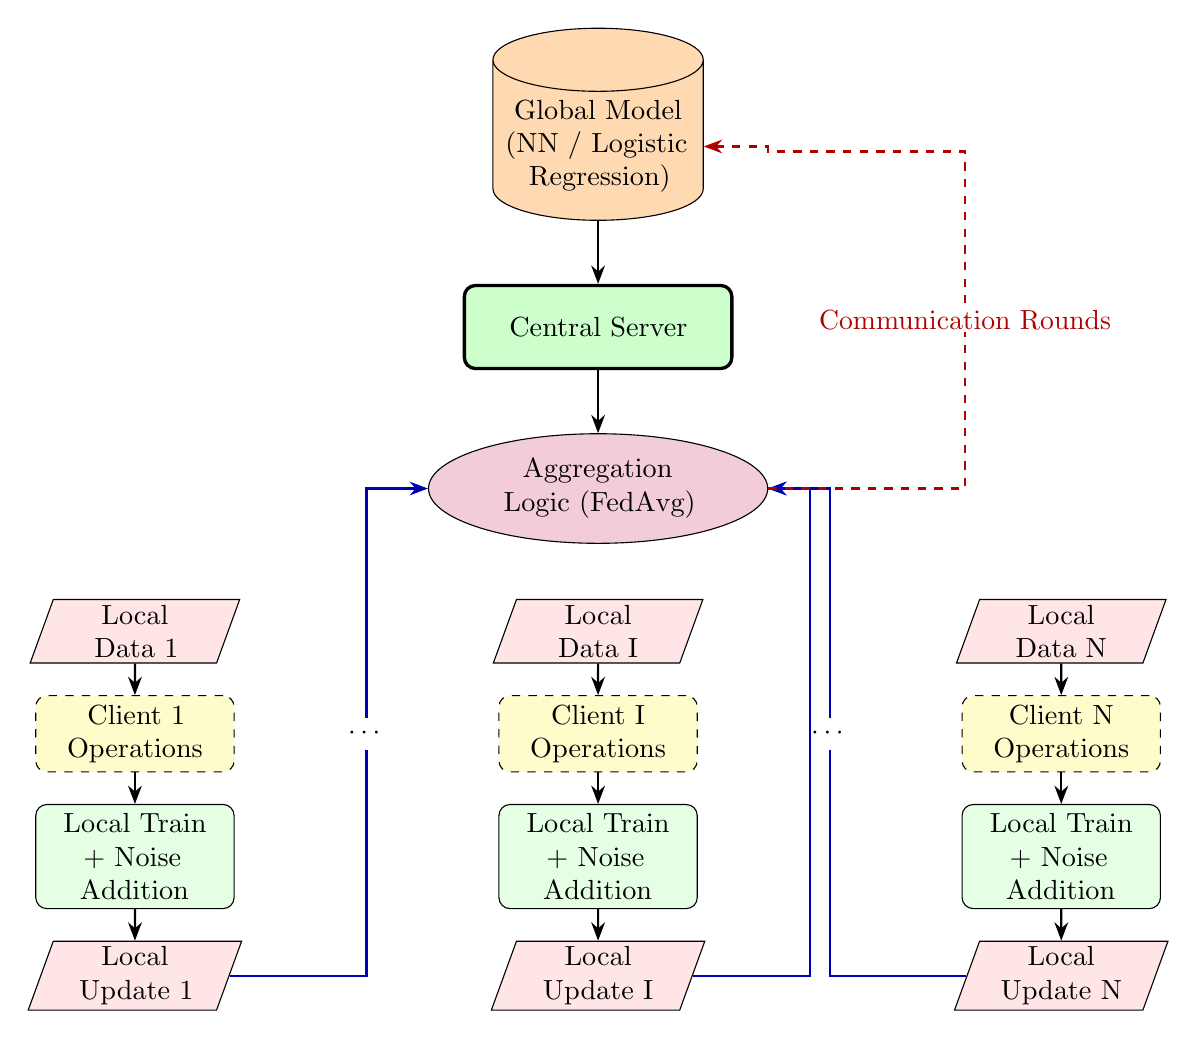
\begin{tikzpicture}[
            node distance=0.7cm and 3.5cm,
            block/.style={rectangle, draw, fill=blue!20, text width=6.5em, text centered, rounded corners, minimum height=2.5em},
            server_block/.style={rectangle, draw, fill=green!20, text width=9em, text centered, rounded corners, minimum height=3em, very thick},
            client_node/.style={rectangle, draw, fill=yellow!20, text width=6.5em, text centered, rounded corners, minimum height=2em, dashed},
            model_store/.style={cylinder, shape border rotate=90, draw, fill=orange!30, aspect=0.3, minimum height=2.5em, text centered, text width=7em, inner sep=3pt},
            data_client/.style={trapezium, trapezium left angle=70, trapezium right angle=110, draw, fill=red!10, minimum height=2em, text width=5.5em, text centered, inner sep=2pt},
            operation/.style={ellipse, draw, fill=purple!20, minimum height=2.5em, text width=8em, text centered},
            dots_style/.style={text width=3em, text centered},
            main_flow_arrow/.style={-Stealth, thick, black},
            client_comm_arrow/.style={-Stealth, thick, blue!70!black},
            loop_arrow/.style={-Stealth, thick, red!70!black, dashed} 
        ]
    
        \node[server_block] (server_core) {Central Server};
        
        \node[model_store, above=0.8cm of server_core] (global_model) {Global Model (NN / Logistic Regression)};
        
        \node[operation, below=0.8cm of server_core] (aggregation) {Aggregation Logic (FedAvg)};
    
        \node[data_client, below=0.7cm of aggregation] (dataI) {Local Data I}; 
            
        \node[client_node, below=0.4cm of dataI] (clientI_ops) {Client I Operations};
        
        \node[block, fill=green!10, below=0.4cm of clientI_ops] (trainI) {Local Train + Noise Addition};
        
        \node[data_client, below=0.4cm of trainI] (updateI) {Local Update I};
    
        \node[data_client, left=of dataI] (data1) {Local Data 1}; 
        
        \node[client_node, below=0.4cm of data1] (client1_ops) {Client 1 Operations};
        
        \node[block, fill=green!10, below=0.4cm of client1_ops] (train1) {Local Train + Noise Addition};
        
        \node[data_client, below=0.4cm of train1] (update1) {Local Update 1};
    
        \node[data_client, right=of dataI,] (dataN) {Local Data N}; 
            
        \node[client_node, below=0.4cm of dataN] (clientN_ops) {Client N Operations};
        
        \node[block, fill=green!10, below=0.4cm of clientN_ops] (trainN) {Local Train + Noise Addition};
        
        \node[data_client, below=0.4cm of trainN] (updateN) {Local Update N};
        
        \node[dots_style] at ($(client1_ops.east)!0.5!(clientI_ops.west)$) (data_dots1) {$\cdots$};
        
        \node[dots_style] at ($(clientI_ops.east)!0.5!(clientN_ops.west)$) (data_dots2) {$\cdots$};
        \draw[main_flow_arrow] (global_model.south) -- (server_core.north);
        \draw[main_flow_arrow] (server_core.south) -- (aggregation.north);
    
        \draw[main_flow_arrow] (data1) -- (client1_ops);
        \draw[main_flow_arrow] (client1_ops) -- (train1);
        \draw[main_flow_arrow] (train1) -- (update1);
        \draw[main_flow_arrow] (dataN) -- (clientN_ops);
        \draw[main_flow_arrow] (clientN_ops) -- (trainN);
        \draw[main_flow_arrow] (trainN) -- (updateN);
        \draw[main_flow_arrow] (dataI) -- (clientI_ops);
        \draw[main_flow_arrow] (clientI_ops) -- (trainI);
        \draw[main_flow_arrow] (trainI) -- (updateI);
    
        \draw[client_comm_arrow] (update1.east) -| (data_dots1) |- (aggregation);
        \draw[client_comm_arrow] (updateN.west) -| (data_dots2) |- (aggregation);
        \draw[client_comm_arrow] (updateI) -| ($(data_dots2.west) + (0.4cm, 0)$) |- (aggregation.east);
    
        \coordinate (agg_output_point) at ($(aggregation.south) + (0,-0.3cm)$);
        \coordinate (global_model_input_point) at ($(global_model.south) + (0,0.3cm)$); 
        
        \draw[loop_arrow] (aggregation.east)
          -- ++(2.5cm,0) 
          -- ++(0,4.28cm)
          node[midway, fill=white, inner sep=1pt, text=red!70!black] {Communication Rounds}
          -- ++(-2.5cm,0) 
          |- (global_model.east); 
    
    
        \end{tikzpicture}
    } 
    \caption{Federated Learning Pipeline}
    \label{fig:fl}
\end{figure*}

\tableofcontents

\begin{abstract}
\small
This report details the development and evaluation of a PoC system for decentralized machine learning pipelines. Such a system enables multiple parties to collaborate in a single model exchanging only locally computed parameter updates, allowing for securing the data, and protecting the privacy of raw datasets. The system implements the Federated Averaging or \textbf{FedAvg} Algorithm. The system includes a server for model aggregation and a client for local training. Noise addition has also been explored, which allows for protection against reverse engineering attacks. The report also provides a comparison of Vanilla ML models, and FL models.
\end{abstract}

\section{Introduction}
The model implemented here is known as Federated Averaging, and the general system is called \textit{Federated Learning} (FL). FL is a distributed machine learning technique where multiple clients collaboratively train a shared model by accessing a central server, without any exchange of their local data. Instead, clients can train a model on their local data and send only the model updates to the server, which aggregates these updates to produce the global state of the model. 

In this \textit{Proof-of-Concept}, we implement the FedAvg algorithm from the foundational principles, without using any libraries designed specifically for the same. We have also partially attempted to consider the various privacy-enhancing mechanisms, such as addition of random noise to client updates, and evaluate the trade-offs between higher noise additions (i.e. more privacy gains) and model performance using metrics such as accuracy, and F1-score.  


\section{Technology Stack}
In choosing the stack for developing the web application, several choices were made. It was clear that the backend needed to be in python. Since the data cannot ever leave the user's device, we had to train the model on the local data by either training the model in the browser itself, by using libraries such as \texttt{TensorFlow.js}, or create a local training client built on top of python, which the user can download and use to compute the model updates locally. 

We decided to go with the local client due to some limitations of a web-based approach. First, computations in the browser are not very efficient, and even though Tensorflow is optimised for the same, ML is just not native to web browsers. Second, we need a way to store the updates locally till all the participants of the Training Group have completed their training. Achieving this requires exploring IndexedDBs or accessing disk storage of the user, both of which defeat the purpose of having a purely web based client. Using a local client which the user can download solves both of these problems.

Also, since there is no weight-age on the UI/UX of the web app, we decided to serve static \texttt{.html} instead of implementing the front end in a proper web framework such as NextJS. To serve these files directly from the backend, built on top of python, we had a choice of using \texttt{flask} or \texttt{django}. Since django comes shipped with pre-existing authorization methods and admin commands, we decided to go with django, allowing for a easier development experience. 

\section{Model Architecture and Design}

\subsection{Centralized ML Pipeline}
A standard centralized machine learning pipeline was used as a baseline for performance comparison. Such a pipeline is illustrated in Fig \ref{fig:vanilla}. The pipeline consists of the following steps. First the centralized dataset undergoes pre-processing. This pre-processed data is then split into Test, Validation and Train datasets, and a single model instance is trained using the training set, with validation set used for hyperparameter tuning. 

\begin{figure}[htbp]
    \centering
    \resizebox{!}{0.35\textheight}{
        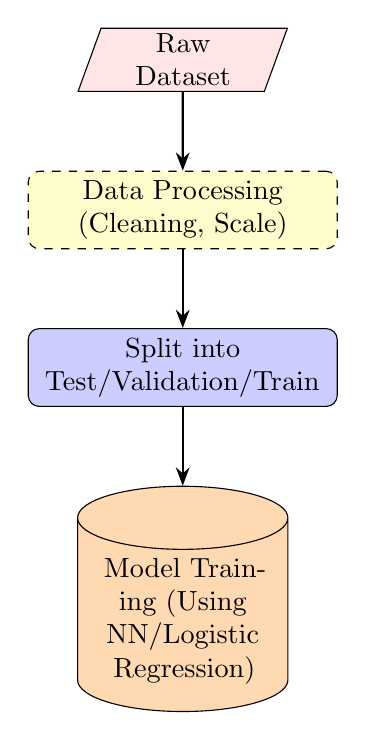
\begin{tikzpicture}[
            block/.style={rectangle, draw, fill=blue!20, text width=10.5em, text centered, rounded corners, minimum height=2.5em},
            data_client/.style={trapezium, trapezium left angle=70, trapezium right angle=110, draw, fill=red!10, minimum height=2em, text width=5.5em, text centered, inner sep=2pt},
            client_node/.style={rectangle, draw, fill=yellow!20, text width=10.5em, text centered, rounded corners, minimum height=2em, dashed},
            server_block/.style={rectangle, draw, fill=green!20, text width=9em, text centered, rounded corners, minimum height=3em, very thick},
            main_flow_arrow/.style={-Stealth, thick, black},
            model_store/.style={cylinder, shape border rotate=90, draw, fill=orange!30, aspect=0.3, minimum height=2.5em, text centered, text width=7em, inner sep=3pt}
        ]

        \node[data_client] (raw_dataset) {Raw Dataset};
        \node[client_node, below=of raw_dataset] (processing) {Data Processing (Cleaning, Scale)};
        \node[block, below=of processing] (split) {Split into Test/Validation/Train};
        \node[model_store, below=of split] (train) {Model Training (Using NN/Logistic Regression)};

        \draw[main_flow_arrow] (raw_dataset) -- (processing);
        \draw[main_flow_arrow] (processing) -- (split);
        \draw[main_flow_arrow] (split) -- (train);
        
        \end{tikzpicture}
    }
    \caption{Normal Pipeline of Training ML Algorithms}
    \label{fig:vanilla}
\end{figure}


\subsection{FL Pipeline and Platform Design}
The FL pipeline diagram can be represented as shown in the Fig \ref{fig:fl}. The pipeline is enabled by a Django-based web application serving as the central coordinator. The server manages user authentication, training group definitions, initializes the global model parameters for each training group, provides an interface for clients to download the current global model weights, and the client-side training script for the selected model. It facilitates an admin user to trigger aggregation, and initialize uninitialized training groups. 

Scripts here are specific to each dataset. Adding a new dataset to the Training Groups would require changing the \texttt{settings.py} file, and adding another config for the dataset, and creating the corresponding local trainer for the dataset. 

There can be as many rounds of a FL Cycle as needed, and there is no fixed requirement for a FL Cycle, except that at least a single active user submission must be available. Any number of users can contribute to a given Training Group, and the number is not limited to just 3. As we will see later, this allows for computation costs to be distributed among many users, and ultimately saves a central agent cost of training the model, since the cost of aggregating a model (which is simply taking averaging), is much lesser than heavy computations such as backpropagation, which are hence off-loaded to sister computer systems.

\subsection{Security and Privacy Measures}
Since the raw-data never leaves the client's devices, the secrecy of sensitive data can be maintained in this environment. Furthermore, adding noise using methods as \textit{Gaussian Noise} after the parameters have been trained locally can help obscure individual contributions, and provide a level of privacy, preventing any agent from effectively reconstructing the data that might've gone into training the parameters. Specifically, the Gaussian Noise is a method in which random values are drawn from a Gaussian or \textit{Normal Distribution}. The \texttt{noise\_scale} parameter in our local trainer decides how much noise will be introduced in our parameters. The \texttt{noise\_scale} is essentially the \textit{Standard Deviation} of the added noise. The more the \texttt{noise\_scale} the more noisy our final data will be.

\section{Implementation Details}
\subsection{Django Backend Implementation}
The backend server forms the coordination point for the FL process. The main django app responsible for the functionalities is \texttt{fl\_platform}. Three key models were defined in the app to handle the FL process effectively. Starting with \textit{TrainingGroup}, which represent a specific dataset. It stores the name, description (optional) and the \texttt{model\_config\_key}, which links the group to a configuration in the \texttt{settings.py} as mentioned earlier. The config has information about the PyTorch model class, the input/output dimension and the client script name. The \textit{GlobalModel} model stores metadata for each version (after a communication round) of a global model. This includes the \texttt{round\_number, FileField}, the model also includes \texttt{accuracy, loss} fields, but they have not been implemented in the views. Finally \textit{ClientUpdateSubmission} records each model update file submitted. The files are stored in subdirectories under \texttt{MEDIA\_ROOT} which in our case is simply \texttt{media}. 

Talking about views, there are standard views for authorization. The key views are implemented in the \texttt{fl\_platform} app. The \texttt{initialize\_global\_model} view instantiates a randomized \texttt{state\_dict()} of the model to a file, and creates a \texttt{GlobalModel} database record for Round 0.  

\subsection{PyTorch Model Definitions}
To keep the simplicity of the app, and since there was no weightage on the sophistication on the implemented ML algorithms, we have only implemented two architectures. The first of them is the \textit{LogisticRegressionModel} which is a simple linear model for binary classification tasks (which in our case include the income, smoking and lumpy datasets), and a \textit{SimpleNN} which is a \textit{Neural Network} with a single hidden layer, by default of size $64$. 

\section{Experimental Setup}
A Google Colab environment was used for all the tests that were conducted. For each dataset, the following splitting strategy was employed, $70\%$ for training, $30\%$ for testing. Training poor was again divided into $70\%$ for training and the rest for validation, resulting in a $49-21-30$ split of the original data. This split was used to train the centralized model. 

The same split was then used to simulate clients, by splitting it into $3$ clients in an \textit{Identically Distributed (IID)} data partitioning scenario. The same global test set for the vanilla model was used to evaluate the performance of the final model. 

\subsection{Model Architectures and Configurations}
For the datasets Income, Lumpy Skin and Smoking Bio-Signals, a \textit{Logistic Regression Model} was used, with a fixed output dimension (since the problems are of binary classification), and an input dimension, determined during pre-processing of each dataset and preset in the config files. For Income Dataset, this number is $96$, for Smoking Dataset, this number is $24$ and for Lumpy Skin, this number is $16$.

Since the Credit Score dataset poses a multi-class classification problem, a simple logistic regression model wouldn't work. Here a \textit{Neural Network} with 1 hidden layer of size $64$ with ReLU activation was used. The input dimension again was determined during pre-processing and turned out to be $49$, and the output dimension is $3$ since there are $3$ credit score classes.

\subsection{Training Hyperparameters}
The optimizer used was Adam. A default learning rate of $0.01$ was used in logistic regression and $0.001$ in the neural network, with a batch size of $64$. Total number of epochs for Income, Lumpy Skin and Smoking datasets were used as $100$, but for Credit Score, it was cutoff at $50$ since little to no variation could be seen after it. For binary classification, the loss function used is \texttt{nn.BCEWithLogitsLoss} and for multi-class task, \texttt{nn.CrossEntropyLoss} was used.

For the FL simulation, number of client was fixed at $3$ per round, and number of communication rounds held were $50$. Same loss functions, optimizers were used. Also, noise scales tested were $0.0$, $0.01$ and $0.05$. 

Finally, the performance was evaluated using the Accuracy, Loss and the F1-Score.

\section{Results and Analysis}
\subsection{Training Results}
\subsubsection{Income Dataset (Logistic Regression)}
The centralized training of the Logistic Regression model on the Adult Income dataset yielded the following performance on the held-out global test set: Test Accuracy: 84.73\%, Test F1-Score: 0.6635, Test Loss: 0.3312. 

The key results on the global test set after 50 communication rounds are summarized in Table \ref{tab:income_fl_results}. illustrates the test accuracy and loss progression over communication rounds for different noise scales.

\begin{table}[hbtp]
  \centering
  \caption{FL Performance on Adult Income Dataset (50 Rounds)}
  \label{tab:income_fl_results}
  \resizebox{\columnwidth}{!}{
    \begin{tabular}{lccc}
        \hline
        Noise Scale ($\sigma$) & Accuracy (\%) & Loss &  Time (s) \\
        \hline
        0.0                   & 84.66      & 0.3393 & 152 \\
        0.01                  & 84.73      & 0.3390 & 152 \\
        0.05                  & 84.52      & 0.3398 & 154 \\
        \hline
    \end{tabular}
  }
\end{table}

\subsubsection{Lumpy Skin Dataset (Logistic Regression)}
The centralized training of the Logistic Regression model on the Lumpy Skin Dataset yielded the following performance on the held-out global test set: Test Accuracy: 93.85\%, Test F1-Score: 0.7315, Test Loss: 0.1756. Time taken to train 30s. 

The key results on the global test set after 50 communication rounds are summarized in Table \ref{tab:lumpy_fl_results}. illustrates the test accuracy and loss progression over communication rounds for different noise scales.

\begin{table}[hbtp]
  \centering
  \caption{FL Performance on Lumpy Skin Dataset (50 Rounds)}
  \label{tab:lumpy_fl_results}
  \resizebox{\columnwidth}{!}{
    \begin{tabular}{lccc}
        \hline
        Noise Scale ($\sigma$) & Accuracy (\%) & Loss &  Time (s) \\
        \hline
        0.0                   & 93.79     & 0.1726 & 85 \\
        0.01                  & 93.93      & 0.1729 & 83 \\
        0.05                  & 93.87      & 0.1731 & 90 \\
        \hline
    \end{tabular}
  }
\end{table}

\subsubsection{Smoking Dataset (Logistic Regression)}
The centralized training of the Logistic Regression model on the Smoking Dataset yielded the following performance on the held-out global test set: Test Accuracy: 74.10\%, Test F1-Score: 0.6649, Test Loss: 0.4849. Time taken to train 78s. 

The key results on the global test set after 50 communication rounds are summarized in Table \ref{tab:smoking_fl_results}. illustrates the test accuracy and loss progression over communication rounds for different noise scales.

\begin{table}[hbtp]
  \centering
  \caption{FL Performance on Smoking Dataset (50 Rounds)}
  \label{tab:smoking_fl_results}
  \resizebox{\columnwidth}{!}{
    \begin{tabular}{lccc}
        \hline
        Noise Scale ($\sigma$) & Accuracy (\%) & Loss &  Time (s) \\
        \hline
        0.0                   & 73.84     & 0.4858 & 189 \\
        0.01                  & 74.06      & 0.4858 & 191 \\
        0.05                  & 74.02      & 0.4856 & 189 \\
        \hline
    \end{tabular}
  }
\end{table}

\subsubsection{Credit Score Dataset (Neural Network)}
The centralized training of the Neural Network model on the Credit Score Dataset yielded the following performance on the held-out global test set: Test Accuracy: 66.40\%, Val Loss: 0.7020. Time taken to train 78s. Note however that this was run only for 50 epochs, as compared to the previous models which were all run for 100 epochs. 

The key results on the global test set after 50 communication rounds are summarized in Table \ref{tab:smoking_fl_results}. illustrates the test accuracy and loss progression over communication rounds for different noise scales.

\begin{table}[hbtp]
  \centering
  \caption{FL Performance on Smoking Dataset (50 Rounds)}
  \label{tab:smoking_fl_results}
  \resizebox{\columnwidth}{!}{
    \begin{tabular}{lccc}
        \hline
        Noise Scale ($\sigma$) & Accuracy (\%) & Loss &  Time (s) \\
        \hline
        0.0                   & 69.92     & 0.6992 & 421 \\
        0.005                  & 67.65     & 0.6929 & 408 \\
        0.02                  & 66.51      & 0.7050 & 423 \\
        \hline
    \end{tabular}
  }
\end{table}

\subsection{Inference}
It may be noticed that the difference in accuracy between FL algorithms and vanilla algorithms is not significant. In some cases, the accuracy for FL algorithms surpasses the accuracy of vanilla models. There can be multiple causes for this, such as more significant data being available first, and hence influencing the model weights the most. Also, there is no fixed direction in which the noise scale affects the accuracy of the models, provided that the scale of the noise is not very high. However, it does increase the instability of algorithms, as can be noticed by looking at figures \ref{fig:income} \ref{fig:lumpy} etc. that the variation in model test accuracy over rounds is higher for high noise scale as compared to low noise scales.  

Another noticeable effect is on the training time. The training times for FL algorithms in these cases appears to be thrice that of the training time for the vanilla case (except in the credit score case, where it looks like it's approximately 6 times the training time). In general as the number of agents increases, the time taken for a FL algorithm to be carried out end to end increases, however, as previously discussed, this computational load is distributed to all of the sister systems and hence does not appear to be significant, and in fact helps utilise unitilised computational power. 
 
\begin{figure*}[t]
    \centering
    \includegraphics[width=\textwidth]{income.png}
    \caption{FL model test accuracy and loss per communication round on Income dataset for different noise scales.}
    \label{fig:income}
\end{figure*}
\begin{figure*}[t]
    \centering
    \includegraphics[width=\textwidth]{lumpy.png}
    \caption{FL model test accuracy and loss per communication round on Lumpy Skin dataset for different noise scales.}
    \label{fig:lumpy}
\end{figure*}
\begin{figure*}[t]
    \centering
    \includegraphics[width=\textwidth]{smoking.png}
    \caption{FL model test accuracy and loss per communication round on Smoking dataset for different noise scales.}
    \label{fig:smoking}
\end{figure*}
\begin{figure*}[t]
    \centering
    \includegraphics[width=\textwidth]{score.png}
    \caption{FL model test accuracy and loss per communication round on Credit Score dataset for different noise scales.}
    \label{fig:score}


\end{figure*}


\section{Conclusion}
In conclusion, this project successfully designed, implemented, and evaluated a Proof of concept (PoC) system for decentralized model training using Federated Learning (FL), specifically the Federated Averaging (FedAvg) algorithm.

\section*{References}
\begin{small}
\begin{enumerate}[label={[{\arabic*}]}]
    \item IBM Research. What is Federated Learning?[\href{https://research.ibm.com/blog/what-is-federated-learning}{Link}]
    
    \item Lumpy Skin Disease Dataset, Kaggle. [\href{https://www.kaggle.com/datasets/saurabhshahane/lumpy-skin-disease-dataset}{Link}]
    
    \item Smoker Status Prediction Using Biosignals, Kaggle. [\href{https://www.kaggle.com/datasets/gauravduttakiit/smoker-status-prediction-using-biosignals}{Link}]
    
    \item Adult Income Dataset, Kaggle. [\href{https://www.kaggle.com/datasets/wenruliu/adult-income-dataset}{Link}]
    
    \item Credit Score Classification, Kaggle. [\href{https://www.kaggle.com/datasets/parisrohan/credit-score-classification}{Link}]
\end{enumerate}
\end{small}

\end{document}
